\section{Construction}
\subsection*{NIPoPoWs}
For our construction, we will use a primitive called Non-Interactive Proofs of
Proof-of-Work recently introduced by Miller et al.~\cite{nipopows}.
Non-Interactive Proofs of Proofs-of-Work are cryptographic protocols which
implement a \emph{prover} and a \emph{verifier}. The prover is a \emph{full
node} on some \emph{remote blockchain} and has full access to that blockchain;
the verifier does not have access access to that blockchain at all. However, the
verifier has access to the genesis block $\mathcal{G}$ of the remote blockchain.
The prover wants to convince the verifier that an \emph{event} took place in the
remote blockchain; for instance, a smart contract method was called with certain
parameter values or that a payment was made into a particular address. The fact
that such an event took place can easily be determined if one inspects the whole
blockchain. However, the prover wishes to convince the verifier by only sending
a \emph{succinct proof}, a short string that is sufficient to convince the
verifier but which does not linearly grow with the size of the remote
blockchain. Succinct proofs are \emph{polylogarithmic} in the size of the remote
blockchain. The verifier further wishes not to be fooled by claims of
\emph{adversarial provers} who provide incorrect proofs, i.e., proving that
event took place while it in fact didn't, or claiming that an event didn't take
place while it actually did. To withstand such attacks, the verifier accepts
multiple proofs, at least one of which is assumed to have been generated by an
honest party. By comparing these proofs with each other, the verifier can
extract a reliable truth value which corresponds to the same value it would
deduce if it were to be itself running a full node on the remote blockchain with
complete access to it. This property is the \emph{security} of NIPoPoWs scheme
and was realized in~\cite{nipopows}.

It is worth noting that, while in this paper we are interested in \emph{events},
the original NIPoPoWs construction talks about general \emph{predicates} that
are evaluated on blockchains. We remark that blockchain events satisfy the
requirements that make a blockchain predicate provable within the NIPoPoWs
framework. In particular, given a particular genesis block $\mathcal{G}$, a
smart contract address \textsf{addr}, an event name \textsf{Event}, and
a series of event parameter values
$(\textsf{param}_1, \textsf{param}_2, \cdots, \textsf{param}_n)$, the predicate
$e$ we wish to check for truth is the following: \emph{Has the event named
\textsf{Event} been fired with parameters $(\textsf{param}_1, \textsf{param}_2,
\cdots, \textsf{param}_n)$ by the smart contract residing in address
\textsf{addr} on the blockchain with genesis block $\mathcal{G}$ at least $k$
blocks ago?} This particular predicate is (1) \emph{monotonic}, meaning that it
starts with the value \textsf{false} and, if it ever becomes \textsf{true}, it
cannot ever change its value back as the blockchain grows; (2)
\emph{infix-sensitive}, meaning that its truth value can be deduced by
inspecting only a constant number of blocks on the blockchain (one block, within
which the event firing was confirmed); and (3) \emph{stable}, meaning that, if
one party deduces that its value is \textsf{true}, then soon enough \emph{all}
other parties will deduce that its value is \textsf{true} (this last property is
due to the requirement that the event be buried under $k$ blocks ensuring a
blockchain reorganization up to $k$ blocks ago cannot affect the predicate's
value).

In order to determine whether an event took place, the NIPoPoW verifier function
\textsf{verify}$^{\mathcal{G},e}_{k,m}(\mathcal{P})$ accepts the event
description in the form of a blockchain predicate $e$, which we gave above, the
genesis block of the remote chain $\mathcal{G}$, as well as two security
parameters $k$ and $m$. These security parameters can be constants specified
when the sidechain system is created and do not need to be modified thereafter.
The NIPoPoWs paper gives concrete value recommendations for these parameters and
so we do not delve into that here. Subsequently, the NIPoPoWs verifier accepts a
set of \emph{proofs} $\mathcal{P} = \{\pi_1, \pi_2, \cdots, \pi_n\}$ which it
compares and extracts a truth value for the predicate: Whether the event has
taken place in the remote blockchain or not. As long as at least one
\emph{honestly generated} proof $\pi_i$ has been provided, the verifier's
security ensures that the output will correspond to whether the event actually
occurred.

\noindent
\textbf{Adoption considerations. } Our sidechain construction has certain
requirements for both the source and the target blockchain to be able to allow
for interoperability between them. For one-way pegs, the requirements are
different for each blockchain. In the case of two-way pegs, both blockchains
must satisfy both the source and the target blockchain requirements listed
below.

\begin{itemize}
  \item \textbf{The source blockchain. } The source blockchain needs to be able
        to support \emph{proofs} about it, which requires augmenting it with an
        \emph{interlink} vector~\cite{popow}. This interlink vector can be added
        to a blockchain using a \emph{velvet fork}~\cite{nipopows,velvet}, which
        can be user-initiated without miner awareness, and so does not require a
        hard or a soft fork. However, if a source blockchain were to be
        augmented with such a structure, it would only allow proving events that
        occur after the structure has started being included.
  \item \textbf{The target blockchain. } The target blockchain needs to be able
        to run the \textsf{verify} function defined above. This function can be
        programmed in a Turing-complete language such as Solidity. If the source
        blockchain proof-of-work hash function can be expressed as an opcode
        within the target blockchain's VM, the way, e.g., Bitcoin's SHA256 hash
        function can be expressed in Solidity\footnote{While SHA256 does not
        strictly constitute an opcode, it is one of Ethereum's `precompiled'
        contracts, which acts similarly.}, the implementation can work. If the
        hash function is not available as an opcode, the gas cost of executing
        proof verification, while asymptotically polylogarithmic, is prohibitive
        in practice.
\end{itemize}

\noindent
\textbf{Remote blockchain agnosticism. }
We underline the remarkable property that miners and full nodes of the target
blockchain do not need to be aware of the source blockchain at all. To them,
all information about the source blockchain is simply a string which is passed
as a parameter to a smart contract and can remain \emph{agnostic} to its
semantics as a proof. Additionally, miners and full nodes of the source
blockchain do not need to be aware of the target blockchain. Only the parties
interested in facilitating cross-chain events must be aware of both. In
particular, those facilitators need to maintain an SPV node on the source
blockchain (requiring that they have downloaded all block headers), with which
they can generate their NIPoPoW, and to broadcast their proof on the target
blockchain, which can be done by connecting to an honest target blockchain node
and relaying the respective transaction containing the NIPoPoW to them, in this
case without downloading the whole target blockchain headers. Finally, another
facilitator must set up the smart contract by broadcasting a transaction on the
target blockchain containing the initialization of the smart contract, including
the genesis block hash of the source blockchain. This last participant does not
need to download any block headers from any blockchain. This property allows
users to initiate sidechain relationships between different blockchains, as long
as the blockchains allow generating proofs about them and validating proofs
about remote blockchains, without designing any opcode specific to any
particular remote blockchain.

\subsection*{Cross-chain events}

We give our \textsf{crosschain} smart contract construction in
Algorithm~\ref{alg.crosschain}. This construction allows for informing one
blockchain about events that took place in another and will form the foundation
for subsequent constructions which will allow proper sidechain transfers of
assets. The \textsf{crosschain} smart contract is parameterized by three
parameters, $k, m, z$. The parameters $k$ and $m$ are the underlying security
parameters of the NIPoPoWs construction. The value $z$ is a \emph{collateral}
parameter, denominated in ether (or the local currency of the blockchain in
which the execution takes place), which is used to incentivize honest
participants to intervene in cases of adversarial claims.

\import{./}{algorithms/crosschain.tex}

The contract can be \emph{inherited} by other contracts that wish to adopt its
functionality. It is used on the target blockchain and it works as follows.
First, the \textsf{initialize} method is called, passing the \emph{hash} of the
genesis block of the remote chain which this contract will handle. This method
is declared \textsf{internal} and can only be called by the contract inheriting
from it. It is intended to be called only once to configure the contract. Users
of the contract can check that it has been configured with the correct genesis
block by its creator prior to using it. We note that it is possible to have a
contract interact with \emph{multiple} remote chains. While the algorithm does
not reflect this in order to keep complexity low, the contract can be extended
in a straightforward manner to include multiple genesis block hashes.

When an event has taken place in the remote blockchain, any source blockchain
SPV node, the \emph{author}, can inform the \textsf{crosschain} contract about
this fact by generating a NIPoPoW $\pi$ claiming that the predicate ensuring
event inclusion is \textsf{true} using their current view of the source
blockchain. This proof can then be submitted to the target blockchain by calling
the \textsf{submit-event-proof} function and passing it the proof $\pi$ and the
event predicate $e$. Submission of proof of a claim that a remote event has
taken place must be accompanied by a collateral payment $z$. If the author
is honest, this collateral will be returned to her later. The
\textsf{submit-event-proof} function runs the NIPoPoW \textsf{verify} algorithm
to check that the proof $\pi$ is well-formed and that its claim is that the
predicate is \textsf{true}. It then stores the proof for later use. It also
stores the address of the \emph{author} and an \emph{expiration block number}.

Upon submission of a valid proof to the \textsf{submit-event-proof} function,
the event is considered \emph{tentatively} accepted for a period of $k$ blocks.
This period is the \emph{contestation period} during which another party, the
\emph{contester} can provide a counter-proof showing that the original proof was
adversarial. This can be done by any party by calling the
\textsf{submit-contesting-proof} function during the contestation period,
passing it the contesting proof $\pi$ and the event predicate $e$. The function
runs the NIPoPoW \textsf{verify} algorithm to compare the original proof
$\textsf{events}[e].\textsf{proof}$ against the contesting proof $\pi$. If the
verification algorithm concludes that the original proof was invalid, the event
is abandoned and the collateral is paid to the contester.

Otherwise, when the contestation period has expired without any valid
contestations, the author can call the \textsf{finalize-event} function, passing
the event predicate $e$. This function changes the acceptance of the event from
tentative to \emph{permanent} by including it in the \textsf{finalized-events}
set and returns the collateral to the author. Finally, the \textsf{event-exists}
function can be used by the inheriting contract by passing the event predicate
$e$ to check if an event has been permanently accepted. The lifecycle of the
scheme scheme is illustrated in Figure~\ref{fig.contestation}.

\begin{figure}
    \caption{The source blockchain's event included in the black box, upon
             sufficient confirmation by $k_1$ blocks (not shown), is transmitted
             to the target blockchain at the bottom. The target blockchain
             includes the event \emph{tentatively} in block $1$ until a
             contestation period of $k_2$ has passed; the event is included
             \emph{permanently} in block $2$; subsequently, permanent inclusion
             needs to be confirmed with $k_2$ further blocks.}
    \centering
    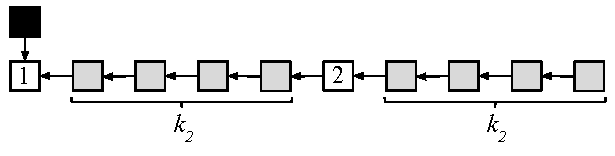
\includegraphics[width=0.6 \columnwidth,keepaspectratio]{figures/contestation.pdf}
    \label{fig.contestation}
\end{figure}

\begin{theorem}[Correctness]
  If an event is emitted on the \emph{source} blockchain, then it will be
  \emph{permanently accepted} into the \emph{target} blockchain by
  Algorithm~\ref{alg.crosschain}.
\end{theorem}
\begin{proof}
  ?
  % TODO
\end{proof}

\begin{theorem}[Security]
  If an event has \emph{not} been emitted on the \emph{source} blockchain, then
  it will \emph{not} be \emph{permanently accepted} into the \emph{target}
  blockchain by Algorithm~\ref{alg.crosschain}.
\end{theorem}
\begin{proof}
  ?
  % TODO
\end{proof}

\subsection*{Two-way pegged sidechains}
Having created the generic crosschain contract, we can now build two-way pegged
sidechains upon it.

First, we note that our purpose of retaining the nature of an asset as it moves
from one blockchain to another is readily achieved if two-way pegging exists. To
be more concrete, assume that we wish to move ether (ETH), the native currency
of the Ethereum blockchain, to the Ethereum Classic blockchain. When it is moved
to the Ethereum Classic blockchain, it will be represented as an ERC20 token
within that blockchain. The ERC20 standard~\cite{erc20} defines an interface
which can be implemented by smart contracts to enable holding and transferring
custom tokens such as ICO tokens. Let's call this custom token ETH20. As long as
it is always possible to move ETH into ETH20 and back at a one-to-one rate, the
nature of the asset is retained as long as the asset is fungible. The economic
reason is that the price of ETH and ETH20 on the market will necessarily be the
same. For, if the price of ETH were to ever be above the price of ETH20 in the
market, then one would exchange their ETH20 for ETH using sidechains and sell
their ETH on the market instead, and vice versa.

The sidechain smart contracts are presented in Algorithm~\ref{alg.sidechain1}
and Algorithm~\ref{alg.sidechain2}. These smart contracts both extend the
\textsf{crosschain} smart contract described in Algorithm~\ref{alg.crosschain}.
Furthermore, Algorithm~\ref{alg.sidechain2} also extends basic ERC20
functionality. We assume the base ERC20 contract allows users who have positive
balances to transfer them between each other, as is done by many popular
implementations~\cite{openzeppelin}. Algorithm~\ref{alg.sidechain1} contains the
\textsf{sidechain}$_1$ contract which will be instantiated on the one blockchain
while Algorithm~\ref{alg.sidechain2} contains the \textsf{sidechain}$_2$
contract and will be instantiated on the other. Suppose the genesis block hash
of the first blockchain is $\mathcal{G}_1$ and of the second blockchain is
$\mathcal{G}_2$. We will use the genesis block hash of each blockchain as its
unique identifier.

\import{./}{algorithms/sidechain.tex}

The two smart contracts each contain an \textsf{initialize} method which accepts
the hash of the remote blockchain as well as the address of the remote smart
contract it will interface with. Note that, while the two genesis hashes can be
hard-coded into the respective smart contract code itself, the remote contract
address cannot be built-in as a constant into the smart contract, but must be
later specified by calling the \textsf{initialize} function. The reason is that,
if \textsf{sidechain}$_1$ were to be created on $\mathcal{G}_1$, it would
require the address of \textsf{sidechain}$_2$ to exist prior to its creation,
and vice versa in a circular dependency. Therefore, the two contracts must first
be created on their respective blockchain to obtain addresses, and then their
\textsf{initialize} methods can be called to inform each contract about the
address of the remote contract. Specifically, first the contract
\textsf{sidechain}$_1$ is created on $\mathcal{G}_1$ to obtain its instance
address which we will also denote \textsf{sidechain}$_1$. Then the second
contract, \textsf{sidechain}$_2$ is created on $\mathcal{G}_2$ to obtain its
address \textsf{sidechain}$_2$. Then, the \textsf{initialize} function of
\textsf{sidechain}$_1$ is called, passing it $\mathcal{G}_2$ and the address
\textsf{sidechain}$_2$. Finally, \textsf{initialize} is called on
\textsf{sidechain}$_2$, passing it $\mathcal{G}_1$ and the address
\textsf{sidechain}$_1$. These initialization parameters are stored by the
respective smart contracts for future use. As the \textsf{crosschain} contract
requires, the \textsf{initialize} method can only be called once. Any user
wishing to utilize this sidechain is expected to validate that the contracts
have been set up correctly and that \textsf{initialize} has been called with the
appropriate parameters.

Following our example with Ethereum and Ethereum Classic, \textsf{sidechain}$_1$
runs on the Ethereum blockchain and \textsf{sidechain}$_2$ runs on the Ethereum
Classic blockchain. \textsf{sidechain}$_1$ contains a \textsf{deposit} function
which is \emph{payable} in the native asset of Ethereum, ETH. When a user pays
ETH into the \textsf{deposit} function, the funds are kept by the smart contract
and can later be used to pay parties who wish to \emph{withdraw}, an operation
which can be performed by calling the \textsf{withdraw} function.
\textsf{sidechain}$_2$ contains similar \textsf{deposit} and \textsf{withdraw}
functions which, however, do not pay in the native currency of Ethereum Classic,
but instead maintain a \textsf{balance} mapping akin to a typical ERC20
implementation. The balance is updated when a user deposits or withdraws.

Moving funds from the Ethereum blockchain into the Ethereum Classic blockchain
works as follows. First, the user pays with ETH to call the \textsf{deposit}
function of \textsf{sidechain}$_1$ which resides on $\mathcal{G}_1$, passing the
\textsf{target} parameter which indicates their address in the Ethereum Classic
blockchain that they wish to receive the money into. This call emits an event,
\textsf{Deposited}$_1$ which contains the necessary data: the \textsf{target},
the \textsf{amount} paid, as well as a unique counter \textsf{ctr} to allow for
future payments of the same amount to the same target. When the event has been
emitted and buried under $k_1$ blocks within the Ethereum blockchain, the user
produces an Ethereum NIPoPoW $\pi_1$ about the predicate $e_1$ which claims that
the event \textsf{Deposited}$_1$ has been emitted in blockchain $\mathcal{G}_1$
with the particular parameters by the contract at address
\textsf{sidechain}$_1$. We will slightly abuse notation for event predicates and
let $e_1$ be specified by the tuple containing the contract address, event name
and parameters $(\textsf{sidechain}_1, \textsf{Deposited}_1, (\textsf{amount},
\textsf{target}, \textsf{ctr}))$, noting that there is an obvious correspondence
between the two.

Subsequently, the user calls the \textsf{submit-event-proof} function of
\textsf{sidechain}$_2$ (which is inherited from the \textsf{crosschain}
contract), passing the NIPoPoW $\pi_1$ and the event predicate $e_1$, paying
collateral $z$, which registers $e_1$ on \textsf{sidechain}$_2$ as tentative.
Because the user is honest, intuitively no adversary can produce a $\pi'_1$
which disproves their claim during the dispute period (we make this statement
more concrete later), and therefore the user waits for $k_2$ blocks for the
contestation period to expire. She then calls the \textsf{finalize-event}
function for $e_1$ and receives back the collateral $z$, marking the event
permanent. Finally, she calls the dual function \textsf{withdraw} of
\textsf{sidechain}$_2$, passing it the same parameters that $e_1$ was issued
with. The \textsf{withdraw} function checks that $e_1$ exists using the
\textsf{event-exists} method, which will return \textsf{true}. The user is then
credited with \textsf{amount} in their ETH20 balance stored in
$\textsf{balances}[\textsf{target}]$. Note that this increment in balance
creates brand new ETH20 tokens.

The user can then move around their ETH20 tokens by utilizing the functionality
inherited by \textsf{sidechain}$_2$ from the \textsf{ERC20} contract. They can
give parts of their tokens to others, receive tokens from others, and so on.
When some (not necessarily the same) user is ready to move some (not necessarily
the same) amount of ETH20 from the Ethereum Classic blockchain back into ETH
on the Ethereum blockchain, they follow the reverse procedure. Specifically,
they call the \textsf{withdraw} function of \textsf{sidechain}$_2$ which ensures
their ERC20 balance is sufficient, deduces the requested amount, and fires an
event $e_2$ as before. At this point, these particular ETH20 tokens are
destroyed by the balance deduction. Once $e_2$ is confirmed in $\mathcal{G}_2$,
the user produces the NIPoPoW $\pi_2$ about the predicate $e_2$ which claims
that a payment was made within $\mathcal{G}_2$. That proof is then submitted to
\textsf{sidechain}$_1$ by calling the \textsf{submit-event-proof} and
\textsf{finalize-event} functions as before. Last, the user calls the
\textsf{withdraw} function of \textsf{sidechain}$_1$, which uses the
\textsf{event-exists} function which will return \textsf{true}, finally paying
back the user the respective amount of ETH. Because the only way to create ETH20
tokens in \textsf{sidechain}$_2$ is by depositing ETH into
\textsf{sidechain}$_1$, there will always exist a sufficient balance of ETH
owned by the \textsf{sidechains}$_1$ smart contract to pay any requested
withdrawals.

% Prove correctness! (through succinctness of NIPoPoWs)
